\RequirePackage{filecontents}
\begin{filecontents}{\jobname.bib}
@MISC{FGV:2020,
  author = {{Fundação Getúlio Vargas (FGV)}},
  title = {Pesquisa Anual do Uso de {TI}},
  year = {2020},
  howpublished = {\url {https://eaesp.fgv.br/ensinoeconhecimento/centros/cia/pesquisa}},
  note = {Acessado em: 20 mai. 2020},
}

@MISC{AdamaAlvo:2020,
  author = {{Adama Brasil}},
  title = {Adama Alvo},
  year = {2020},
  howpublished = {\url {https://www.adama.com/brasil/pt/adama-inovacao/adama-alvo}},
  note = {Acessado em: 29 mai. 2020}
}

@ARTICLE{Ribeiro:2018,
  AUTHOR = {Josiana Gonçalves Ribeiro and Douglas Yusuf Marinho and Jose Waldo Martínez Espinosa},
  TITLE = {Agricultura 4.0: Desafios à Produção de Alimentos e Inovações Tecnológicas},
  JOURNAL = {Simpósio de Engenharia de Produção},
  YEAR = {2018},
  URL = {https://files.cercomp.ufg.br/weby/up/1012/o/AGRICULTURA_4.0_DESAFIOS_%C3%80_PRODU%C3%87%C3%83O_DE_ALIMENTOS_E_INOVA%C3%87%C3%95ES_TECNOL%C3%93GICAS.pdf}
}

@ARTICLE{Rose:2019,
  AUTHOR = {Rose, David Christian and Chilvers, Jason},
  TITLE = {Agriculture 4.0: Broadening Responsible Innovation in an Era of Smart Farming},
  JOURNAL = {Frontiers in Sustainable Food Systems},
  VOLUME = {2},
  PAGES = {87},
  YEAR = {2018},
  URL = {https://www.frontiersin.org/article/10.3389/fsufs.2018.00087},       
  DOI = {10.3389/fsufs.2018.00087},      	
  ISSN = {2571-581X},   
  ABSTRACT = {Agriculture is undergoing a new technology revolution supported by policy-makers around the world. While smart technologies, such as Artificial Intelligence, robotics, and the Internet of Things, could play an important role in achieving enhanced productivity and greater eco-efficiency, critics have suggested that the consideration of social implications is being side-lined. Research illustrates that some agricultural practitioners are concerned about using certain smart technologies. Indeed, some studies argue that agricultural societies may be changed, or “re-scripted,” in undesirable ways, and there is precedent to suggest that wider society may be concerned about radical new agricultural technologies. We therefore encourage policy-makers, funders, technology companies, and researchers to consider the views of both farming communities and wider society. In agriculture, the concept of responsible innovation has not been widely considered, although two recent papers have made useful suggestions. We build on these interventions by arguing that key dimensions of responsible innovation—anticipation, inclusion, reflexivity, and responsiveness—should be applied to this fourth agricultural revolution. We argue, however, that ideas of responsible innovation should be further developed in order to make them relevant and robust for emergent agri-tech, and that frameworks should be tested in practice to see if they can actively shape innovation trajectories. In making suggestions on how to construct a more comprehensive framework for responsible innovation in sustainable agriculture, we call for: (i) a more systemic approach that maps and attends to the wider ecology of innovations associated with this fourth agricultural revolution; (ii) a broadening of notions of “inclusion” in responsible innovation to account better for diverse and already existing spaces of participation in agri-tech, and (iii) greater testing of frameworks in practice to see if they are capable of making innovation processes more socially responsible.}
}

@ARTICLE{Shepherd:2018,
  DOI = {10.1002/jsfa.9346},
  URL = {https://doi.org/10.1002/jsfa.9346},
  YEAR = {2018},
  MONTH = {Oct},
  PUBLISHER = {Wiley},
  AUTHOR = {Mark Shepherd and James A Turner and Bruce Small and David Wheeler},
  TITLE = {Priorities for science to overcome hurdles thwarting the full promise of the `digital agriculture' revolution},
  JOURNAL = {Journal of the Science of Food and Agriculture}     
}

@INPROCEEDINGS{Souza:2017,
  AUTHOR = {Souza, Leonardo Antonio Martins and Sotsek, Nicolle Christine},
  YEAR = {2017},
  MONTH = {11},
  TITLE = {Indústria 4.0: uma revisão sistemática da literatura nacional},
  DOI = {10.14488/ENEGEP2017_TN_STO_238_376_31632},
  BOOKTITLE = {XXXVII Encontro Nacional de Engenharia de Produção}
}

@INPROCEEDINGS{Massruha:2017,
  AUTHOR = {Silvia Maria Fonseca Silveira Massruhá and Maria Angelica de Andrade Leite},
  YEAR = {2017},
  TITLE = {Agro 4.0 - rumo à agricultura digital},
  PAGES = {28-35},
  BOOKTITLE = {Embrapa Informática Agropecuária}
}

@ARTICLE{Zhai:2020,
  title = "Decision support systems for agriculture 4.0: Survey and challenges",
  journal = "Computers and Electronics in Agriculture",
  volume = "170",
  pages = "105256",
  year = "2020",
  issn = "0168-1699",
  doi = "https://doi.org/10.1016/j.compag.2020.105256",
  url = "http://www.sciencedirect.com/science/article/pii/S0168169919316497",
  author = "Zhaoyu Zhai and José Fernán Martínez and Victoria Beltran and Néstor Lucas Martínez",
  keywords = "Agriculture, Smart farming, Decision-making, Decision support systems",
  abstract = "Undoubtedly, high demands for food from the world-wide growing population are impacting the environment and putting many pressures on agricultural productivity. Agriculture 4.0, as the fourth evolution in the farming technology, puts forward four essential requirements: increasing productivity, allocating resources reasonably, adapting to climate change, and avoiding food waste. As advanced information systems and Internet technologies are adopted in Agriculture 4.0, enormous farming data, such as meteorological information, soil conditions, marketing demands, and land uses, can be collected, analyzed, and processed for assisting farmers in making appropriate decisions and obtaining higher profits. Therefore, agricultural decision support systems for Agriculture 4.0 has become a very attractive topic for the research community. The objective of this paper aims at exploring the upcoming challenges of employing agricultural decision support systems in Agriculture 4.0. Future researchers may improve the decision support systems by overcoming these detected challenges. In this paper, the systematic literature review technique is used to survey thirteen representative decision support systems, including their applications for agricultural mission planning, water resources management, climate change adaptation, and food waste control. Each decision support system is analyzed under a systematic manner. A comprehensive evaluation is conducted from the aspects of interoperability, scalability, accessibility, usability, etc. Based on the evaluation result, upcoming challenges are detected and summarized, suggesting the development trends and demonstrating potential improvements for future research."
}

@ARTICLE{Gutierrez:2019,
  title = "A review of visualisations in agricultural decision support systems: An {HCI} perspective",
  journal = "Computers and Electronics in Agriculture",
  volume = "163",
  pages = "104844",
  year = "2019",
  issn = "0168-1699",
  doi = "https://doi.org/10.1016/j.compag.2019.05.053",
  url = "http://www.sciencedirect.com/science/article/pii/S0168169918319069",
  author = "Francisco Gutiérrez and Nyi Nyi Htun and Florian Schlenz and Aikaterini Kasimati and Katrien Verbert",
  keywords = "Decision support systems, Human-computer interaction, Information visualisation, Precision agriculture",
  abstract = "Decision Support Systems (DSSs) are used in precision agriculture to provide feedback to a variety of stakeholders, including farmers, advisers, researchers and policymakers. However, increments in the amount of data might lead to data quality issues, and as these applications scale into big, real-time monitoring systems the problem gets even more challenging. Visualisation is a powerful technique used in these systems that provides an indispensable step in assisting end-users to understand and interpret the data. In this paper, we present a systematic review to synthesise literature related to the use of visualisation techniques in the domain of agriculture. The search identified 61 eligible articles, from which we established end-users, visualisation techniques and data collection methods across different application domains. We found visualisation techniques used in various areas of agriculture, including viticulture, dairy farming, wheat production and irrigation management. Our results show that the majority of DSSs utilise maps, together with satellite imagery, as the central visualisation. Also, we observed that there is an excellent opportunity for dashboards to enable end-users with better interaction support to understand the uncertainty of data. Based on this analysis, we provide design guidelines towards the implementation of more interactive and visual DSSs."
}

@ARTICLE{Walling:2020,
  title = "Developing successful environmental decision support systems: Challenges and best practices",
  journal = "Journal of Environmental Management",
  volume = "264",
  pages = "110513",
  year = "2020",
  issn = "0301-4797",
  doi = "https://doi.org/10.1016/j.jenvman.2020.110513",
  url = "http://www.sciencedirect.com/science/article/pii/S0301479720304473",
  author = "Eric Walling and Céline Vaneeckhaute",
  keywords = "Environmental decision support system, Decision-making, Evaluation, Development challenges, Stakeholders, Best practices",
  abstract = "Environmental decision support systems (EDSSs), or DSS applied in the environmental field, have been developed for over 40 years now. However, most of these tools fail to find use or fall out of use extremely quickly. In the aim of aiding in the conception and development of practical and successful decision support systems, i.e. systems that can lead to positive outcomes, this review looks over the existing literature, both EDSS-centric and from broader decision-related fields, to highlight some of the most important challenges influencing the success and usability of these systems. In all, 13 major challenges facing EDSS development were identified and over 60 recommendations and best practices were provided to address these challenges. Though this paper is mainly focused on environmental decision support systems, most of the highlighted information and conclusions are applicable to the development of decision support systems in any field."
}

@ARTICLE{Rupnik:2019,
  title = "AgroDSS: A decision support system for agriculture and farming",
  journal = "Computers and Electronics in Agriculture",
  volume = "161",
  pages = "260 - 271",
  year = "2019",
  note = "BigData and DSS in Agriculture",
  issn = "0168-1699",
  doi = "https://doi.org/10.1016/j.compag.2018.04.001",
  url = "http://www.sciencedirect.com/science/article/pii/S0168169917314205",
  author = "Rok Rupnik and Matjaž Kukar and Petar Vračar and Domen Košir and Darko Pevec and Zoran Bosnić",
  keywords = "Decision support system, Agriculture, Farming, 68U35, 68T05",
  abstract = "Decision support systems, data analysis and data mining have become significant tools for improving business in professional world. The emerging technologies are making the precision agriculture omnipresent and allow potential for enriching it with computer-assisted decision support systems for farm management. In this paper we describe a novel system AgroDSS that bridges the gap between agricultural systems and state-of-the-art decision support methodology. The described system is intended for integration into the existing farm management information systems and provides a cloud-based decision support toolbox, allowing farmers to upload their own data, utilize several data analysis methods and retrieve their outputs. The implemented tools include predictive modeling with explanation, accuracy evaluation, time series clustering and decomposition, and structural change detection. They can help users make predictions for simulated scenarios and better understand the dependencies (interactions) within their domain. We apply the AgroDSS system on a case study of pest population dynamics, illustrating the potential for its use."
}

@ARTICLE{Lundstrom:2018,
  title = "Considering farmers' situated knowledge of using agricultural decision support systems ({AgriDSS}) to Foster farming practices: The case of {CropSAT}",
  journal = "Agricultural Systems",
  volume = "159",
  pages = "9 - 20",
  year = "2018",
  issn = "0308-521X",
  doi = "https://doi.org/10.1016/j.agsy.2017.10.004",
  url = "http://www.sciencedirect.com/science/article/pii/S0308521X17303906",
  author = "Christina Lundström and Jessica Lindblom",
  keywords = "Precision agriculture, Agricultural decision support systems, Sustainable intensification, Distributed cognition, Learning, Care",
  abstract = "Precision agriculture is an important part of the sustainable intensification of agriculture, where information and communications technology and other technologies are necessary, but not sufficient for sustainable farming systems. The technology must fit into farmers' practice and be handled by their experienced-based, situated knowledge in order to contribute to increased sustainability in their farming. This study analysed the relationship between farmers' experience-based situated knowledge and the use of agricultural decision support systems in order to develop care by farmers in their practice. The theoretical framework of distributed cognition was used as a lens when investigating and analysing farmers' use of an agricultural decision support system called CropSAT developed for calculation of variable rate application files for nitrogen fertilisation from satellite images. In the case study, the unit of analysis was broadened to the whole socio-technical system of farmers' decision-making and learning, including other people and different kinds of tools and artefacts. The results revealed that social contexts could support farmers' development of cognitive strategies for use of agricultural decision support systems, e.g. CropSAT, and could thus facilitate decision-making and learning through development of enhanced professional vision that hopefully may increase farmers' situated knowledge and care in PA."
}

@techreport{Kitchenham:2004,
  added-at = {2009-04-28T08:33:13.000+0200},
  address = {Department of Computer Science, Keele University, UK},
  author = {Kitchenham, Barbara},
  biburl = {https://www.bibsonomy.org/bibtex/2e48137ec01b6308876e05ab1ecdf4bc4/wiljami74},
  description = {systematic literature review},
  interhash = {75c82aef0bd6a41e833647512d5e78d6},
  intrahash = {e48137ec01b6308876e05ab1ecdf4bc4},
  institution = {Keele University},
  keywords = {systematic_literature_review},
  timestamp = {2011-03-24T14:57:31.000+0100},
  title = {Procedures for Performing Systematic Reviews},
  type = {Keele University. Technical Report TR/SE-0401},
  year = 2004
}

@misc{ONU:2020,
  author = {{Organização das Nações Unidas}},
  title = {17 objetivos para transformar o nosso mundo},
  howpublished = {\url {https://nacoesunidas.org/pos2015/agenda2030/}},
  year =  {2020},
  note = {Acessado em: 29 mai. 2020}
}

@book{Torres:2013,
  author = {Gabriel Torres},
  publisher = {NovaTerra},
  title = {Hardware},
  year = {2013}
}
\end{filecontents}

\documentclass[12pt]{article}
\usepackage{class/sbc-template}
\usepackage{graphicx,url}
\usepackage[utf8]{inputenc}
\usepackage[brazil]{babel}
\usepackage{multirow}
\usepackage{hyperref} 
\usepackage{abntex2cite}

\bibliographystyle{sbc}
     
\sloppy

\title{Um estudo sobre sistemas colaborativos eficientes para os usuários no contexto da Agricultura 4.0}

\author{Diogo C. T. Batista\inst{1}, Cléber G. Corrêa\inst{1}, Letícia M. Peres\inst{2}, Roberto Pereira\inst{2}}

\address{Universidade Tecnológica Federal do Paraná (UTFPR)\\
  Cornélio Procópio -- Paraná -- Brasil
	\nextinstitute
	Universidade Federal do Paraná (UFPR)\\
	Curitiba -- Paraná -- Brasil
	\email{diogo@diogocezar.com,clebergimenez@utfpr.edu.br,\{lmperes,rpereira\}@inf.ufpr.br}
	}


\begin{document} 

\maketitle
     
\begin{resumo} 
A Agricultura 4.0 explora a utilização de tecnologias computacionais de ponta, envolvendo a Agricultura e Pecuária de Precisão, bem como a Agricultura Digital, que empregam a automação, a robótica agrícola, \textit{Big Data}, a Internet das Coisas, entre outras. A utilização dessas tecnologias busca uma produção agrícola eficiente e sustentável, possibilitando, por exemplo, a economia de água na irrigação ou de insumos na adubagem dos solos. Entretanto, o acesso aos recursos necessários para a exploração dessas tecnologias não é a realidade de grande parte do setor agrícola. Além disso, a resistência na adoção de novas tecnologias é um problema ainda em aberto. Este trabalho busca a exploração de métodos, técnicas e ferramentas, que direcionem soluções computacionais inseridas no contexto da Agricultura 4.0, com o intuito de apoiar o desenvolvimento de sistemas nesta área. Para isso, propõe-se um estudo em Engenharia de Software para projetar, implementar e avaliar sistemas computacionais, colaborativos e eficientes na realização de tarefas por parte dos profissionais ou usuários da área agrícola.\\

\textbf{Palavras-chave:} Agricultura 4.0; Sistemas Colaborativos; Sistema de Apoio a Decisão; Smartphones.
\end{resumo}

\section{Introdução}
\label{sec:introducao}

São grandes os desafios relacionados à utilização de tecnologias digitais como ferramentas de apoio ao trabalho humano de forma eficiente, eficaz e justa \cite{Rose:2019}. Para isso, a humanidade apoia-se nas descobertas e comprovações de milhares de anos da comunidade científica, que proporcionam resultados relevantes, alcançados por meio da exploração das técnicas e métodos descobertos e aprimorados ao longo dos anos.

A indústria é um exemplo de como essa evolução aconteceu. Seu marco se dá com a definição da Era Artesanal, na qual, os bens e serviços eram criados por um único indivíduo: o artesão. Este era responsável por deter todo o conhecimento dos métodos e processos para a fabricação de um produto ou para a prestação de um serviço. Com a criação e o aperfeiçoamento das máquinas a vapor, estes processos puderam ser minimamente automatizados, e isso deu origem a Primeira Revolução Industrial. A Segunda Revolução Industrial, acontece com a utilização da eletricidade e principalmente dos processos que possibilitaram a implantação da produção em massa idealizadas por Henry Ford. A Terceira Revolução Industrial se inicia após a Segunda Guerra Mundial, com o descobrimento e a utilização da robótica e do uso de computadores para a automação das indústrias \cite{Souza:2017}.

Mais recente, muito tem se falado sobre a Quarta Revolução Industrial, que surge em 2011 na Alemanha, com a proposta de oferecer para a indústria o que há de mais moderno em automação e sistemas inteligentes, possibilitando uma série de melhorias como por exemplo: a redução dos custos, a economia de energia e o aumento da segurança. Essas e outras melhorias têm sido exploradas por meio da utilização de ferramentas e tecnologias como: \textit{Big Data}, \textit{Analytics}, Serviços de Nuvem, Impressões 3D, Segurança Cibernética, Robôs Autônomos, Internet das Coisas, Sensores sem Fio, Realidade Aumentada, Simulação, Integração Horizontal e Integração Vertical \cite{Souza:2017}.

Além da indústria, outro setor que evoluiu muito ao longo dos anos foi a agricultura. A agricultura foi fundamental para alavancar o desenvolvimento das civilizações ao longo da história, possibilitando que comunidades nômades se estabilizassem em determinadas regiões, explorando técnicas agrícolas para a produção de seu sustento. Entretanto, o cenário atual é bem diferente dos enfrentados pelas primeiras civilizações, o crescimento populacional, e a tendência das pessoas a se tornarem cada vez mais exigentes com o que é consumido, gera um grande desafio para o setor agrícola, que precisa se posicionar eficientemente para atender estas demandas. Dessa forma, novas técnicas têm sido exploradas, e estas, compõem o termo Agricultura 4.0. Estas técnicas utilizam os mesmos métodos e processos inovadores já explorados pela Indústria 4.0, incluindo: a automação, a robótica, \textit{Big Data} e Internet Das Coisas, em um contexto de Agricultura e Pecuária de Precisão e Agricultura Digital \cite{Ribeiro:2018}.

A utilização de componentes tecnológicos não é uma novidade na agricultura, a exploração, por exemplo, de tecnologias como o \textit{Global Positioning System} (GPS), estão presentes a algum tempo na linha de produção agrícola, conhecida como Agricultura de Precisão. A Agricultura 4.0 expande as possibilidades de explorações tecnológicas, com a utilização por exemplo de: \textbf{Sensores}; que possibilitam a coleta automática de dados sobre o solo e clima; \textbf{Veículos Aéreos Não Tripulados (VANTs ou drones) ou Satélites}, que podem apresentar recursos de imagem cada vez mais avançados, auxiliando no aumento de produtividades e ajudando a reduzir danos às lavouras, visto que possibilitam o monitoramento em tempo real; \textbf{smartphones}, que proporcionam uma interface de entrada e saída de dados rápida, acessível e conhecida por usuários de dispositivos eletrônicos \cite{Shepherd:2018}.

A Agricultura 4.0, com a utilização de sistemas de apoio à decisões, pode levar à produções mais eficientes e ao consumo mais inteligente e sustentável. Entretanto, essa transição não é uma tarefa trivial. Segundo \citeonline{Rose:2019}, a utilização destas ferramentas tecnológicas devem mudar a forma como os agricultores interagem com suas plantações, com isso, cada vez menos os trabalhadores precisão colocar a ``mão na massa'', mudando a forma de como sempre interagiram com seu ofício. E isso pode dificultar a adesão de novas tecnologias. A utilização das técnicas relacionadas a agricultura de precisão demonstraram certa resistência por parte dos agricultores \cite{Rose:2019}. Entretanto, o uso em larga escala de Inteligência Artificial (IA), robótica e outras inovações emergentes, tem o claro potencial de causar consequências sociais não intencionais, imprevistas e indesejadas. Por este motivo, é importante focar em uma parte fundamental para o sucesso da aplicação de novas tecnologias: o usuário. Adicionalmente, podem ser múltiplos usuários, colaborando para realizar determinadas tarefas.

Grande parte das tecnologias adotadas pela Agricultura 4.0 está inserida (pelo menos em algum momento) em um sistema computacional. Sabe-se que um sistema computacional é basicamente composto pela \textit{entrada de dados}, o seu \textit{processamento} e a disponibilização dos seus \textit{resultados}. As duas últimas etapas dependem da qualidade da fonte de dados, ou seja, da entrada das informações \cite{Torres:2013}.

No âmbito agrícola, por mais automatizados que possam estar os processos de obtenções dos dados, com sensores automáticos ou análise de imagens, por exemplo, há dois principais pontos que podem aumentar ainda mais a resistência à adoção das tecnologias: \textit{Indisponibilidade de Equipamentos} e \textit{Conhecimento Empírico}. No cenário atual, não são todos os agricultores que podem destinar parte do seu faturamento para a aquisição de equipamentos modernos que facilitariam a coleta de dados. Além disso, existe uma variável de grande importância que deve ser inserida na equação da Agricultura 4.0, a experiência do agricultor com a sua propriedade e a sua área de atuação. Segundo \citeonline{Rose:2019} aproximar o usuário final do processo tecnológico, pode ser uma estratégia eficiente para a adoção de novas tecnologias. Dessa forma, pode ser necessária a adaptação de métodos, técnicas e ferramentas da Engenharia de Software, permitindo projetar, implementar e avaliar sistemas colaborativos eficientes para a Agricultura 4.0.

O presente projeto pode contribuir com determinados \textit{Objetivos de Desenvolvimento Sustentável}, descritos pela Organização das Nações Unidas \cite{ONU:2020}. No documento da organização, são descritos 17 objetivos que buscam concretizar os direitos humanos e promover a igualdade. Para isso, tais objetivos e metas foram definidos com o intuito de estimular ações para os próximos 15 anos, em áreas de importância crucial para a humanidade e para o planeta. Dentre os objetivos, dois deles têm relação direta com este trabalho:

\begin{itemize}
	\item \textit{Objetivo 2: Fome zero e agricultura sustentável} - Aumentar a eficiência da produção agrícola é consequência direta da proposta deste trabalho. A criação de sistemas colaborativos eficientes podem auxiliar na área, promovendo uma produção agrícola sustentável;
	\item \textit{Objetivo 12: Consumo e produções sustentáveis} - Neste quesito, o trabalho contribui com a proposta de uma solução eficiente, acessível (utilizando um \textit{smartphone} como equipamento, por exemplo) e sem a necessidade da aquisição de novos equipamentos para integrações tecnológicas.
\end{itemize}

\section{Objetivo}
\label{sec:objetivo}

A proposta deste projeto é a exploração de métodos, técnicas e ferramentas, que direcionem soluções computacionais inseridas no contexto da Agricultura 4.0, com o intuito de apoiar o desenvolvimento de sistemas nesta área. Para isso, um estudoem Engenharia de Software para projetar, implementar e avaliar sistemas computacionais, colaborativos e eficientes, para auxiliar os usuários na realização de tarefas.

A motivação para o presente trabalho consiste no crescimento da Agricultura 4.0, formada por diversos sistemas computacionais, bem como múltiplos usuários, que podem colaborar entre si de forma eficiente usando essas tecnologias para realizar tarefas. Dessa forma, métodos, técnicas e ferramentas da Engenharia de Software devem ser estudados
para verificar suas aplicações no projeto, implementação e avaliação de sistemas desse tipo.

A \textbf{colaboração} é uma questão importante a ser abordada, pois permite múltiplos usuários trabalhem em um mesmo problema para resolução, esse assunto é argumento na Seção \ref{sec:analise_critica_relevancia}

A \textbf{eficiência} das métricas e metodologias a serem propostas pelo trabalho, deverão passar por um processo de comprovação melhor detalhado na Seção \ref{sec:metodos_materiais}. Para isso, após definição do objeto de estudo principal do trabalho, deve-se desenvolver uma solução que aplique as métricas e diretrises identificadas como hipóteses, com o intúito de realizar a comprovação de sua eficiência e eficácia.

\section{Trabalhos Relacionados}
\label{sec:trabalhos_relacionados}

O trabalho de \citeonline{Zhai:2020} apresenta como desafios para os sistemas de apoio a decisão agrícola: a simplificação de interfaces gráficas dos usuários e utilização de conhecimento dos especialistas do domínio do sistema. Além disso, são abordadas alternativas às entradas de dados comuns, como por exemplo: a utilização do reconhecimento de voz ou a utilização gestos. Outro ponto importante está relacionado ao processo de extração das informações da fonte de dados. Modelos tridimensionais, análise de imagens ou vídeos, e imagens interativas podem ser pontos ainda a serem explorados no contexto em que este trabalho se aplica. Para completar, a colaboração entre usuários também é pouco explorada.

\citeonline{Gutierrez:2019} demonstram por meio da comparação de trabalhos, que a utilização de diversas fontes de informações de entradas é um ponto desejável para a automatização e autonomia na Agricultura 4.0. As principais comparações estão relacionadas às formas de visualização de dados processados. As entradas dos dados são tratadas de forma superficial, bem como a colaboração entre os usuários. Os autores reafirmam a preocupação do presente trabalho em inserir diversas dimensões em uma mesma fonte de dados, e que o processo de obtenção de dados refiånados pode aprimorar os resultados obtidos.

Nos trabalhos de \citeonline{Walling:2020} e \citeonline{Lundstrom:2018} é mostrada a importância da participação do usuário no processo de obtenção de dados. Profissionais com a experiência de seu domínio, são capazes de enriquecer toda a cadeia de inferência nos sistemas de apoio a decisão, independente do domínio de conhecimento no qual os sistemas estão inseridos. Com esses estudos, fica claro que a participação multidisciplinar em toda a cadeia dos sistemas de apoio a decisão podem fazer uma diferença expressiva nos resultados.

O sistema AgroDSS, explorado por \citeonline{Rupnik:2019}, é um exemplo de sistema em que a maioria dos dados coletados é baseada apenas em informações inseridas por meio de formulários de atributos textuais.

\section{Análise Crítica e Relevância}
\label{sec:analise_critica_relevancia}

No cenário agrícola, são vários os papéis dos profissionais que compõem toda a cadeia de produção. A obtenção dos dados utilizados nos sistemas computacionais de apoio à agricultura deve levar em consideração a diversidade de usuários, como agricultores, técnicos agrícolas, engenheiros agrônomos, entre outros. As experiências desses múltiplos profissionais poderiam ser utilizadas para os sistemas computacionais. Por exemplo, para uma nova praga identificada em uma folha de soja, o \textbf{agricultor} poderia inserir as informações relacionadas as suas experiências, como por exemplo se já houve alguma praga com indícios semelhantes aos encontrados, a quanto tempo, por quanto tempo, e como foi resolvido. Enquanto que o \textbf{engenheiro agrônomo} poderia inserir para esta mesma entrada informações extraídas de sua experiência em outras fazendas, colaborando para solucionar o problema de identificação dessa praga. Dessa forma consegue-se extrair diversas \textbf{dimensões} a partir de uma única entrada de dados \cite{Walling:2020}.

Segundo uma pesquisa divulgada pela Fundação Getúlio Vargas (FGV-SP), o Brasil tem hoje dois dispositivos digitais por habitante, incluindo \textit{smartphones}, computadores, \textit{notebooks} e \textit{tablets} \cite{FGV:2020}. Nesse sentido, o país teria aproximadamente 420 milhões de aparelhos digitais ativos. Dessa forma, fica bastante claro que estes dispositivos já fazem parte do dia a dia de muitas pessoas, inclusive dos que fazem parte de toda a cadeia agrícola, sejam agricultores de pequeno e médio portes.

A utilização de \textit{smartphones} e computadores propõe uma solução acessível para um dos pontos mencionados em \citeonline{Rose:2019}, que argumentam que é necessário ampliar as noções de ``inclusão'' em inovação responsável para atender às diversas formas de como os agricultores devem interagir com as fazendas inteligentes. Estes dispositivos já fazem parte da rotina de trabalho do público alvo, não sendo necessários outros investimentos ou aquisições, e ainda assim, possibilitando a inclusão desse público em novas ferramentas criadas para a Agricultura 4.0.

No cenário proposto pela Agricultura 4.0, grande parte dos trabalhos evidenciam que as informações que alimentam os sistemas, podem ser obtidas de forma automatizada, através de sensores ou pela análise de imagens, por exemplo. Entretanto, nem sempre essa é uma realidade aplicável a todos, pelo alto custo e difícil aderência. Outros sistemas, mesmo que completos em termos de sensores e outros recursos tecnológicos, utilizam ainda, entrada manual de informações por parte dos seus usuários, normalmente por meio de formulários com campos pré definidos (comumente dados no formato texto). Sensores e outros recursos também exigem monitoramento de energia, manutenção e desempenho.

\section{Problema a ser Investigado}
\label{sec:problema_investigado}

O principal problema de pesquisa a ser tratado por este trabalho está relacionado a questões sobre como projetar, implementar e avaliar sistemas computacionais colaborativos eficientes para apoiar a tomada de decisão dos usuários no domínio da Agricultura 4.0, usando métodos, técnicas e ferramentas da Engenharia de Software.

Os seguintes tópicos resumem em linhas gerais, quais são os problemas a serem explorados durante o desenvolvimento do projeto:

\subsection{Acesso às Tecnologias}
\label{subsec:acesso_tecnologias}

Grande parte dos trabalhos, na literatura, como demontrado em \cite{Massruha:2017} possuem o foco nos processos de análise e apoio a decisão. Estes trabalhos de pesquisa, normalmente, são suportados por grandes instituições (como Universidades ou empresas privadas) que provêm recursos (como sensores ou drones) para a captação de dados no desenvolvimento dos experimentos. Com tais recursos, os experimentos tendem a focar nos processos que geram os resultados e consequentemente demonstram a eficiência e a eficácia das técnicas propostas pela Agricultura 4.0. Entretanto essa não é a realidade de grande parte dos agricultores, como argumenta \cite{Rose:2019}. Os estudos propostostos por este trabalho, ajudam a resolver o problema da falta de acessibilidade aos recursos necessários para obtenção de dados, permitindo, mesmo que de uma forma menos eficiente e automatizada, a utilização de tecnologias da Agricultura 4.0 por qualquer usuário da cadeia agícola que possua apenas um \textit{smartphone}.

\subsection{Participação Ativa na Colaboração}
\label{subsec:participacao_ativa_colaboracao}

No âmbito agrícola, é bastante comum termos grandes áreas de plantio. Mapear toda a área com dispositivos automatizados poderia gerar um custo muito grande para os agricultores, principalmente com a necessidade de manutenção dos equipamentos que captam as informações dos campos, bem como o consumo de energia elétrica por estes dispositivos. Nesse cenário o presente trabalho também atua na pesquisa de alternativa que possibilitem envolver os fazendeiros no processo de obtenção dos dados. Isso poderia ser feito utlizando a sua experiência e conhecimento de sua propriedade para intuitivamente direcionar a coleta de dados em áreas que pudessem apresentar uma anomalia.

\subsection{Arguição dos Especialistas}
\label{subsec:arquicao_especialistas}

A utilização de recursos automatizados como drones ou sensores tendem a facilitar muito o processo de obtenção de dados em uma fazenda que aplica técnicas da Agricultura 4.0. Tratando de cenários nos quais essa já seja uma realidade, estes recursos automatizados normalmente apenas armazenam uma representação da realidade obtida em algum instante. Por exemplo, um sensor de umidade, poderia registrar os índices de umidade do solo a cada hora. Ou ainda, um drone, poderia fotografar uma área com baixa produtividade. Estes dados não levam em consideração alguns aspectos que poderiam ser enriquecidos com a arguição de um especialista, por exemplo um agrônomo. Por este motivo, este trabalho propõe a investigação de técnicas que possibilitem a inclusão de novas dimensões na coleta de dados, unindo por exemplo, a obtenção automática da umidade do solo com informações e experiências de agrônomos especialistas, que poderiam, por exemplo, informar que apesar de uma leitura de umidade ter ficado fora da expectativa, isso foi advento de uma anormalidade, por ele observada. Como há mais de um especialista em uma mesma tarefa, regras de colaboração devem ser especificadas.

Para os cenários nos quais se utiliza a captação automática dos dados, boa parte das abordagens visto em \cite{Massruha:2017} fazem essa captura de forma contínua e initerruptamente, propondo abordagens que tratem grandes volumes de dados. Esta abordagem por gerar grandes custos, inserindo, por exemplo, dados muitos parecidos que não ajudam na inferência nos resultados dos sistemas de apoio a decisão. Ao utilizar tratativas com mais dimensões, criando por exemplo visões diferentes de agricultores, técnicos agrícolas ou engenheiros agrônomos sobre uma mesma entrada de dados, poderia ajudar na obtenção de dados mais refinados e consequentemente na economia de recursos para manter a coleta automatizada.

\subsection{Interações Manuais}
\label{subsec:interacoes_manuais}

Quando se trata de agricultura, há diversos tipos de cenários. Existem diversos tipos de plantações: soja, milho, café, entre outros. Cada plantação possui suas particularidades. Em cenários nos quais uma plantação apresente vegerações mais densas, entende-se como um problema a captação automática de evidências que comprovem a presença de algum tipo de praga. Essencialmente, a presença dos agricultores e fazendeiros, no dia a dia, analisando as plantações é essencial para o acompanhamento do seu processo produtivo. Uma vegetação densa, poderia esconder uma praga de uma foto aérea feita por um drone, por exemplo. No trabalho proposto, busca-se uma alternativa a este cenário, permitindo a inclusão manual destas informações que podem ser importantes para análise de inferências de apoio a decisão.

\subsection{Experiência e Interface para Colaboração}
\label{subsec:experiencia_interface_colaboracao}

A experiência do usuário com um dispositivo computacional pode influenciar diretamente na adoção de novas tecnologias ou sistemas. É bastante comum a resistência por parte de novos usuários na adoção de sistemas que ainda não tiverem contato. Como objeto de estudos deste trabalho, propõe-se ainda, descobertas relacionadas ao entendimento do perfil do público alvo, e a criação e exploração de personas, que representem os usuários e suas peculiaridades. Criando, desta forma, interfaces que possam ser objetivas, claras, atrativas e principalmente funcionais. Outro desafio a ser explorado é a interação multi-dimensional da entrada de dados, que propõe-se ser refinada, simultaneamente, por diversos colaboradores e que resultem em uma única fonte de dados, possibilitando a inferência de apoio a decisão extraídas de dados refinados e alinhados com as realidades do cenário agrícola apontado por parte da cadeia que já atua na manutenção desta propriedade.

No apêndice \ref{ape:problemas} estão listados, de forma expandandia estes e outros possíveis problemas a serem analisados.

No apêncide \ref{ape:cenario_possivel} ilustra-se um possível cenário, com a utilização de um aplicativo hipotético aplicando alguns dos conceitos a serem explorados pelo trabalho.

\section{Métodos e Materiais}
\label{sec:metodos_materiais}
		
Os métodos para a realização da pesquisa incluem:

\begin{itemize}
	\item Projeto e desenvolvimento de protótipos de sistemas computacionais (aplicativos) para validação;
	\item Planejamento, organização e execução de experimentos envolvendo usuários, normalmente com a utilização de questionários para coletar opiniões referentes as percepções desses usuários na interação humano-computador, bem como no levantamento de requisitos, para verificar a importância das informações de entrada;
	\item Revisão da literatura, podendo utilizar métodos formais de pesquisa, como a revisão sistemática, que fornece um protocolo para o levantamento bibliográfico \cite{Kitchenham:2004};
	\item Análise de resultados utilizando testes estatísticos para verificar a significância das diferenças entre os grupos amostrais comparados (Friedman, ANOVA – Análise da Variância, t-test, Wilcoxon, Mann-Whitnney etc); e estatística descritiva (principalmente gráficos). Os testes estatísticos dependem das características dos dados (normalidade da distribuição, homogeneidade das variâncias, independência e aleatoriedade na coleta etc) e oferecem intervalos de confiança para a análise.
\end{itemize}

Métodos, técnicas e ferramentas de Engenharia de Software serão estudados para uso no trabalho, auxiliando no projeto e desenvolvimento dos protótipos.

Os materiais consistem em \textit{smartphones}, dos próprios usuários; bem como serviços de nuvem para processamento das informações adicionadas pelos usuários. Uma avaliação da aquisição de determinados sensores para medição de informações, tais como temperatura e umidade do solo, será realizada. Adicionalmente, informações de terceiros podem ser empregadas, tais como imagens de satélites e de sítios eletrônicos sobre o clima. 		

A cultura foco provavelmente será a de soja, devido a parceria da UTFPR com a Empresa Brasileira de Pesquisa Agropecuária (Embrapa), situada em Londrina, que trabalha principalmente com a produção da soja. A Embrapa é uma empresa pública de pesquisa vinculada ao Ministério da Agricultura, Pecuária e Abastecimento do Brasil. O seu principal objetivo é a viabilização de soluções provenientes de pesquisas, além do desenvolvimento para a sustentabilidade da agricultura em benefício da sociedade brasileira. A parceria atualmente visa o desenvolvimento de dois sistemas:

\begin{itemize}
	\item Sistema para identificação de pragas, doenças e plantas daninhas da cultura de soja, com suporte \textit{web} e dispositivos móveis. A utilização de imagens capturadas pelos usuários é um dos requisitos do sistema;

	\item Sistema para acompanhamento do crescimento da planta de soja, apresentando os estádios fenológicos, com suporte \textit{web} e dispositivos móveis. A utilização de modelos tridimensionais e vídeos para saída de informações ou visualização por parte dos usuários está prevista. Exemplo de alguns estádios fenológicos da soja podem ser observados na Figura \ref{fig:estadios_fenelogicos}.
\end{itemize}

\begin{figure}
	\centering
  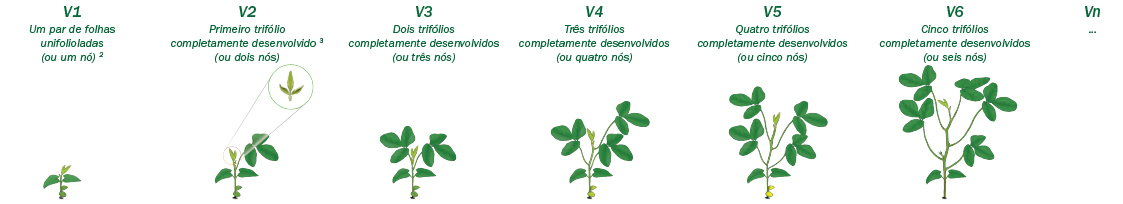
\includegraphics[scale=0.5]{images/EstadiosFenologicos.png}
  \caption{Alguns dos estádios fenológicos da planta da soja (Embrapa).}
  \label{fig:estadios_fenelogicos}
\end{figure} 

Esses sistemas ou módulos desses sistemas poderão ser empregados em estudos de caso, servindo como protótipos para validação, se necessários. 

\section{Plano de Trabalho e Cronograma}
\label{sec:plano_trabalho_cronograma}

O plano de trabalho é composto pelas seguintes atividades principais, dispostas no cronograma apresentado na Tabela \ref{tab:cronograma}, separadas por quadrimestres de cada ano:

\begin{enumerate}
	\item Obtenção de créditos, cursando disciplinas;
	\item Estudo de métodos para mapeamento ou revisão sistemática, permitindo o levantamento de trabalhos na literatura, bem como métodos, técnicas e ferramentas da Engenharia de Software para o desenvolvimento de protótipos;
	\item Estudo do estado da arte, considerando sistemas computacionais colaborativos para dispositivos móveis voltados para a Agricultura 4.0 e seus usuários;
	\item Especificação de cenários;
	\item Exame de proficiência de língua estrangeira;
	\item Exame de qualificação;
	\item Especificação de um sistema computacional para dispositivos móveis, indicando a arquitetura do sistema e principais desafios no desenvolvimento;
	\item Implementação de protótipo para validação;
	\item Testes envolvendo usuários;
	\item Redação de artigos científicos a serem submetidos aos principais eventos e periódicos da área de interesse;
	\item Redação da tese;
	\item Defesa.
\end{enumerate}

As atividades e os períodos serão ajustados conforme o edital do Programa de Pós-Graduação em Informática da UFPR.

\begin{table}[htbp]
	\centering
		\begin{tabular}{|c|c|c|c|c|c|c|c|c|c|c|c|c|}
		\hline
		\multirow{2}{*}{AT} & \multicolumn{3}{c|}{\textbf{Ano 1}} & \multicolumn{3}{c|}{\textbf{Ano 2}} & \multicolumn{3}{c|}{\textbf{Ano 3}} & \multicolumn{3}{c|}{\textbf{Ano 4}} \\ \cline{2-13} 
												& Q1         & Q2         & Q3        & Q1         & Q2         & Q3        & Q1         & Q2         & Q3        & Q1         & Q2         & Q3        \\ \hline
		1                   & •          & •          & •         &            &            &           &            &            &           &            &            &           \\ \hline
		2                   &            &            &           & •          &            &           &            &            &           &            &            &           \\ \hline
		3                   &            &            &           & •          & •          & •         & •          &            &           &            &            &           \\ \hline
		4                   &            &            &           &            & •          &           &            &            &           &            &            &           \\ \hline
		5                   &            &            &           &            & •          &           &            &            &           &            &            &           \\ \hline
		6                   &            &            &           &            & •          &           &            &            &           &            &            &           \\ \hline
		7                   &            &            &           &            & •          &           &            &            &           &            &            &           \\ \hline
		8                   &            &            &           &            &            & •         & •          & •          &           &            &            &           \\ \hline
		9                   &            &            &           &            &            &           &            &            &           & •          &            &           \\ \hline
		10                  &            &            &           &            &            & •         & •          & •          & •         & •          & •          & •         \\ \hline
		11                  &            &            &           &            &            &           &            &            & •         & •          & •          & •         \\ \hline
		12                  &            &            &           &            &            &           &            &            &           &            &            & •         \\ \hline
		\end{tabular}
	\caption{Cronograma de Execução das Atividades}
	\label{tab:cronograma}
\end{table}

Com o objetivo de manter a constante comunicação, e principalmente o acompanhamento e direcionamento das atividades, reuniões semanais devem ser realizadas. Estas reuniões podem ser realizadas de forma presencial (quando possível) ou por meio de vídeo chamadas.

\section{Resultados Esperados}
\label{sec:resultados_esperados}

Pretende-se com o estudo levantar métodos, técnicas e ferramentas de Engenharia de Software para o projeto, implementação e avaliação de sistemas computacionais colaborativos eficientes no contexto da Agricultura 4.0, permitindo que usuários realizem tarefas para aumentar a produção agrícola de forma sustentável.

Espera-se, por fim, a submissão de artigos para conferências e periódicos científicos da área de Ciência da Computação para publicação, como o \textit{ACM Computing Surveys}, \textit{Computer Graphics and Applications}, \textit{Journal on Interactive Systems}, \textit{Computers and Electronics in Agriculture}, \textit{Symposium on Applied Computing}, Simpósio Brasileiro de Engenharia de Software.

\bibliography{\jobname}

\appendix

\section{Problemas de Pesquisa}
\label{ape:problemas}

A seguir lista-se características de sistemas colaborativos (gerais e específicos), relacionadas entre sí, e seus possíveis problemas:

\begin{itemize}
	\item \textbf{atualização em tempo real} - Problemas: múltiplos acessos simultâneos; necessidade de exibição de alertas e erros sobre atrasos; regras de funcionamento (entrada, processamento e saída);
	\item \textbf{múltiplos dispositivos para entrada e saída de dados} - Por exemplo: smartphones, desktops, sensores e robôs. Problemas: integração; interoperabilidade; escalabilidade de dispositivos; tolerância a falhas - possibilidade de substituição de sensores danificados;
	\item \textbf{múltiplos usuários} - Por exemplo: agricultores, técnicos agrícolas, engenheiros agrônomos. Problemas: usabilidade (facilidade de uso, segurança, satisfação, acessibilidade, memorização do usuário), envolvendo interfaces humano-computador e formas de interação; definição de grupos de usuários; carga cognitiva (muitas tecnologias e formas de uso); escalabilidade de usuários; regras de uso; atribuição de significado e interpretação das informações;
	\item \textbf{múltiplas plataformas das fontes de entrada} - Por exemplo: diveras plataformas de smartphones. Problemas: integração; interoperabilidade; usabilidade (facilidade de uso, segurança, satisfação, acessibilidade, memorização do usuário), envolvendo interfaces humano-computador e formas de interação;
	\item \textbf{múltiplos tipos de informações de entrada} - Por exemplo: imagens, voz, texto e vídeos. Problemas: armazenamento e processamento (imagens podem ocupar mais espaço), usabilidade (facilidade de uso, segurança, satisfação, acessibilidade, memorização), envolvendo interfaces humano-computador e formas de interação; carga cognitiva (muitas tecnologias e formas de uso;
	\item \textbf{múltiplos tipos de informações de saída} - Por exemplo: imagens, áudio, texto, modelos tridimensionais e vídeos. Problemas: armazenamento e processamento, usabilidade (facilidade de uso, segurança, satisfação, acessibilidade, memorização), envolvendo interfaces humano-computador e formas de interação; carga cognitiva (muitas tecnologias e formas de uso);
	\item \textbf{múltiplas informações sobre o domínio} - Por exemplo: planta, clima, pragas, ervas daninhas, doenças. Problemas: especificação de subdomínios; granularidade (sistema incorpora informações em atualizações); relação dos subdomínios – planta e clima, planta, pragas e clima);
	\item \textbf{informações de entradas de múltiplos usuários} - Por exemplo: agricultores, técnicos agrícolas, engenheiros agrônomos. Problemas: problemas de conexão com a Internet em regiões afastadas; de consumo de energia; de prioridade dependendo do nível do usuário e do nível de grupo de usuários do mesmo nível; de necessidade de diferentes interfaces humano-computador e formas de interação; de necessidade de definição de níveis e grupos; de processamento e armazenamento local, envolvendo o que pode ser processado e armazenado localmente de acordo com os recursos de hardware e software, o consumo de energia, de maneira a não prejudicar a entrada de novas informações
	\item \textbf{informações de saídas para múltiplos usuários} - Por exemplo: agricultores, técnicos agrícolas, engenheiros agrônomos. Problemas: de usabilidade (facilidade de uso, segurança, satisfação, acessibilidade, memorização), preferências dos usuários, envolvendo interfaces humano-computador e formas de interação);
	\item \textbf{informações de entradas de múltiplos sensores e robôs} - Problemas: conexão com a Internet em regiões afastadas; de nível de autonomia; de consumo de energia; de processamento e armazenamento local, envolvendo o que pode ser processado e armazenado localmente de acordo com os recursos de hardware e software, o consumo de energia, de maneira a não prejudicar a entrada de novas informações)
	\item \textbf{priorização das informações do domínio} - Por exemplo: o processamento de determinadas informações tem prioridade. Por exemplo, uma atividade de colheita está em andamento e o processamento de informações sobre o clima tem prioridade sobre o processamento de informações sobre pragas, no entanto, pode-se perder inferências. Problemas: necessidade da participação de usuários para definição de prioridades; da inviabilidade devido a quantidade de informações e necessidade de agrupamento (clusters) de informações por data, região, clima, tipo da informação, fonte, ou combinação (região e clima); flexibilidade na combinação de informações)
	\item \textbf{sincronização das informações de entrada na nuvem (cloud computing), que  envolve:}
		\begin{itemize}
			\item \textbf{priorização da informação a ser processada: a mesma informação é recebida pelo servidor ao mesmo tempo de diferentes fontes} - Por exemplo: do sensor A e do usuário 1. Problemas: identificação das similaridades; definição de prioridades com a participação de usuários;
			\item \textbf{complementação da informação: a mesma informação é recebida pelo servidor ao mesmo tempo de diferentes fontes} - Exemplo: sensor A e do usuário 1), mas de diferentes tipos (texto, imagem e voz), e elementos podem ser extraídos para completar ou confirmar a informação. Problemas: identificação das diferenças, extração e complemento; custo/benefício da  confirmação em termos de processamento, recursos utilizados;
			\item \textbf{completude da informação} - Por exemplo: a informação é recebida pelo servidor, mas incompleta, como por exemplo, uma imagem incompleta. Problemas: identificação das lacunas e correção, por aproximação, interpolação, utilização de um outro tipo de informação, adoção de um padrão, emissão de avsios para usuários sobre a necessidade de completar a informação – dependência de conexão com a Internet, energia, processamento; custo/benefício de cada forma de completude)
			\item \textbf{informação adicional automática} - Por exemplo: uma informação adicional é adicionada automaticamente em uma informação capturada pelo usuário. Por exemplo, o usuário captura uma imagem usando o smartphone, e o sistema busca automaticamente a geolocalização e o clima. Problemas: conexão com a Internet em regiões afastadas; de consumo de energia; de processamento e armazenamento local, envolvendo o que pode ser processado e armazenado localmente de acordo com os recursos de hardware e software, o consumo de energia, de maneira a não prejudicar a entrada de novas informações);
			\item \textbf{classificação da informação após o processamento} - Por exemplo: informação foi útil, parcialmente útil ou inútil, atribuindo nível de qualidade para a informação. Problemas: custo/benefício para a classificação; de necessidade da participação de usuários; da inviabilidade devido a quantidade de informações e necessidade de agrupamento (clusters) de informações por data, região, clima, tipo da informação, fonte, ou combinação (região e clima); flexibilidade na combinação de informações);
		\end{itemize}
\end{itemize}

\section{Cenário Possível}
\label{ape:cenario_possivel}

Para ilustrar as possibilidades a serem exploradas, descreve-se a utilização de um aplicativo em um cenário hipotético, no qual:

\begin{enumerate}
	\item Um fazendeiro, motivado pelo desconhecimento de uma praga, captura uma imagem de um inseto em uma planta de soja usando seu \textit{smartphone};
	\item A imagem pode receber informações adicionais no próprio \textit{smartphone}, tais como: anotações da quantidade, nome do inseto, enfatizando o tamanho do inseto e o estádio fenológico da planta;
	\item Ainda na imagem, pode ser possível a inclusão de anotações ou destaques em pontos que pudessem ser circulados, pelo fazendeiro, demonstrando pontos de atenção que pudessem ser analisados;
	\item Um engenheiro agrônomo, parceiro deste fazendeiro, analisa a mesma imagem em seu próprio perfil do aplicativo, de forma remota, inserindo e/ou complementando informações sobre o cenário investigado;
	\item Todas as imagens poderiam servir de fonte de dados: a original, a com as anotações do fazendeiro e do engenheiro agrônomo;
	\item Por conta de uma possível dificuldade de conexão (muito comum no cenário rural) o envio das informações poderia não acontecer imediatamente. Mas a operação pode ser marcada como sucesso, deixando essa atividade uma fila de execução em \textit{background};
	\item O próprio sistema registra as coordenadas de geolocalização bem como o momento (horário/dia) desta captura ou oferece a possibilidade de inserção manual destas informações (prevendo a instabilidade da conexão);
	\item Ao receber as informações, um sistema computacional em nuvem, pode relacionar as imagens recebidas com uma ou mais imagens aéreas, capturadas por veículos aéreos não tripulados da mesma região onde está a planta, ou regiões adjacentes em um ou mais momentos anteriores, buscando por insetos. O sistema computacional pode registrar dia e horário de captura da imagem, de modificação, de envio com sucesso;
	\item O sistema computacional pode ainda utilizar utilizar bases de informações compartilhadas entre diferentes regiões e usuários aumentando o refinamento na inferência das informações de apoio a decisão.
\end{enumerate}

\end{document}